\documentclass[10pt,a4paper]{article}

\usepackage[margin=16mm]{geometry}
\usepackage[T1]{fontenc}
\usepackage{helvet}
\usepackage{microtype}
\usepackage{xcolor}
\usepackage{enumitem}
\usepackage{tikz}
\usetikzlibrary{arrows.meta,positioning}

\renewcommand{\familydefault}{\sfdefault}
\pagestyle{empty}
\setlength{\parindent}{0pt}
\setlength{\parskip}{4pt}
\setlist[itemize]{leftmargin=5mm,itemsep=2pt,topsep=2pt}

\definecolor{heading}{HTML}{17365D}
\definecolor{accent}{HTML}{217C7E}
\definecolor{linegray}{HTML}{64748B}
\definecolor{lightgray}{HTML}{F3F5F7}

\newcommand{\briefsection}[1]{%
  \vspace{2pt}%
  {\large\bfseries\color{heading}#1}\par
  \vspace{1pt}%
}

\begin{document}

{\LARGE\bfseries\color{heading} IoT Big-Data Management for TinyML IDS Telemetry}\par
\vspace{2pt}
{\large A course project built on verified intrusion-detection telemetry from IoT boards}\hfill
{\small Nishant Harkut}

\vspace{4pt}
\hrule

\briefsection{Project idea}
My earlier work deployed compact intrusion-detection models on an ESP32-C3 and an Arduino R4 WiFi. Those executions produced trustworthy telemetry such as model predictions, confidence values, device inference time, communication delay, retries, and device status. This project builds the data-management layer required to ingest, process, store, verify, and analyze such telemetry when it is produced continuously by many IoT devices. It does not train a new machine-learning model.

\briefsection{System flow}

\begin{center}
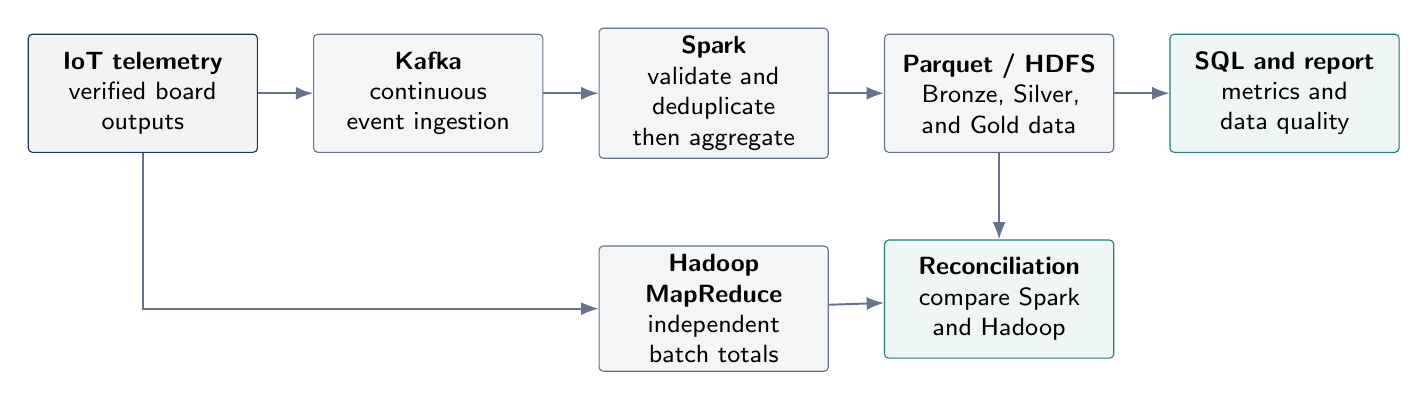
\begin{tikzpicture}[
  font=\small,
  box/.style={draw=linegray, rounded corners=1.5pt, fill=lightgray, align=center,
              minimum height=15mm, text width=27mm, inner sep=3pt},
  primary/.style={box, draw=heading, fill=heading!6},
  final/.style={box, draw=accent, fill=accent!7},
  flow/.style={-{Latex[length=2.2mm]}, line width=0.7pt, draw=linegray}
]
  \node[primary] (source) {\textbf{IoT telemetry}\\verified board outputs};
  \node[box, right=7mm of source] (kafka) {\textbf{Kafka}\\continuous event ingestion};
  \node[box, right=7mm of kafka] (spark) {\textbf{Spark}\\validate and deduplicate\\then aggregate};
  \node[box, right=7mm of spark] (lake) {\textbf{Parquet / HDFS}\\Bronze, Silver,\\and Gold data};
  \node[final, right=7mm of lake] (output) {\textbf{SQL and report}\\metrics and data quality};

  \draw[flow] (source) -- (kafka);
  \draw[flow] (kafka) -- (spark);
  \draw[flow] (spark) -- (lake);
  \draw[flow] (lake) -- (output);

  \node[box, below=11mm of spark] (hadoop) {\textbf{Hadoop MapReduce}\\independent batch totals};
  \node[final, below=11mm of lake] (check) {\textbf{Reconciliation}\\compare Spark and Hadoop};

  \draw[flow] (source.south) |- (hadoop.west);
  \draw[flow] (hadoop) -- (check);
  \draw[flow] (lake) -- (check);
\end{tikzpicture}
\end{center}

\briefsection{Role of Big Data Management}
\begin{itemize}
  \item \textbf{Ingestion and velocity:} Kafka receives continuous events from multiple device streams and preserves delivery metadata.
  \item \textbf{Data quality:} Spark handles duplicates, delayed or out-of-order events, and malformed records. Invalid records are retained separately instead of being silently discarded.
  \item \textbf{Distributed storage and querying:} Parquet and HDFS store telemetry efficiently. Bronze preserves received deliveries, Silver contains validated events, and Gold contains finalized aggregates for SQL analysis.
  \item \textbf{Correctness:} Hadoop MapReduce recomputes exact totals independently. Reconciliation detects missing, duplicated, or altered records in the streaming result.
\end{itemize}

\briefsection{Demonstration and scalability}
The base evidence contains four board-model execution lineages. Each lineage covers the same 56,301 predictive rows, giving 225,204 physical executions in total. These are repeated hardware executions, not 225,204 independent samples. The demonstration will replay the records as a stream and deliberately inject duplicate, late, and malformed deliveries. The output will show how each record moves through validation, quarantine, deduplication, storage, aggregation, and independent verification.

Scalability is demonstrated by increasing the number of simulated device streams and replay rounds without changing the original evidence. For example, five complete replay rounds produce 1,126,020 Kafka deliveries. This is a controlled load test of the data pipeline. In a real deployment, data volume grows with the number of devices, event rate, and operating time.

\briefsection{Expected outcome}
The result is a reproducible IoT big-data pipeline that converts verified TinyML IDS outputs into auditable operational and security analytics. It directly demonstrates Kafka streaming, Spark processing, HDFS and Parquet storage, Hadoop batch verification, SQL analysis, and data-quality handling in one project.

\end{document}
